\documentclass[journal]{IEEEtran}

% *** OPTIONAL PACKAGES ***
\usepackage{cite}
\usepackage[pdftex]{graphicx}
\usepackage[cmex10]{amsmath}
\usepackage[portuguese]{babel}
\usepackage[utf8]{inputenc}
%\usepackage{algorithmic}
%\usepackage{array}
%\usepackage[caption=false,font=footnotesize]{subfig}
%\usepackage{fixltx2e}
%\usepackage{stfloats}
%\usepackage{url}
%\usepackage{hyperref}

% correct bad hyphenation here
\hyphenation{op-tical net-works semi-conduc-tor}

\begin{document}

\title{Robô Recepcionista \\
	Pioneer P5-DX}

\author{\large Pioneer 5 \normalsize \\
Pedro Isidro - 67220,
~Diogo Silva - 75136,
~João Pedrosa - 79833}

% The paper headers
\markboth{Sistemas Autónomos - 2013/2014 - 1\textsuperscript{o} Semestre}{Instituto Superior Técnico}

% make the title area
\maketitle

\begin{abstract}
Abstract (summary of the work)
\end{abstract}

% Note that keywords are not normally used for peerreview papers.
\begin{IEEEkeywords}
Pioneer P5-DX, ROS, autónomo.
\end{IEEEkeywords}

\section{Introdução}
% start with \IEEEPARstart{first letter}{rest of first word}
%Introduction and Motivation (brief description of what the project was about and the motivation for the topic)

Os requisitos para do nosso projecto exigiam ter um robô Pioneer P3-DX capaz de executar tarefas modeladas por uma máquina de estados finitos. Essas tarefas incluem o robô ser capaz de mapear, auto-localiza-se e navegar o seu ambiente e deslocar-se para diferentes localizações indicadas através de interação com utilizadores.

A nossa motivação foi ter um robô recepcionista capaz de receber visitantes num edifício, e.g. um bloco de escritórios. O robô seria capaz de mapear o edício \emph{a priori} para futura utilização, de receber um conjunto de coordenadas já conhecidas (e.g. escritórios de certas pessoas) associadas a palavras-chave, de interagir com utilizadores através de síntese e reconhecimento de voz e, por fim, de guiar os mesmos aos seus destinos.

Durante a implementação do projecto simplificámos algumas destas funcionalidades, nomeadamente o mapeamento e o reconhecimento de voz. O mapeamento foi executado apenas no quinto piso da Torre Norte do IST. O reconhecimento de voz foi restringido a um pequenos dicionário para reduzir a complexidade e a necessidade de adaptar modelos acústicos e treinamento.

%The requirements for our project were having a Pioneer P3-DX capable of carrying out tasks modeled through a Finite State Automaton consisting of mapping, self-localizing and navigating its environment and move to different locations indicated by user interaction.

%Our motivation was to have a receptionist robot, capable of greeting visitors in a big building such as an office block. The robot would be capable of mapping the building \emph{a priori}, receive a set of known coordinates such as people's offices associated with keywords, interact with users through speech synthesis and voice recognition and  guide visitors to their desired destinations.

%During the implementation of the project we simplified on some of these functionalaties, e.g. mapping only the fifth floor of the IST's North Tower and the voice commands were only single word phrases - mostly numbers.
 
\hfill December 6, 2013

\section{Algoritmos e Implementação}
%Methods and Algorithms (brief explanation of the methods used and ROS packages/algorithms used - this is mainly to make sure you understood the conceptual and the implementation part, and to introduce notation - do not write like in a book or tutorial paper) 

\subsection{Mapeamento}
%gmapping - mapping and SLAM using odometry
%
%map\_server - save map and serve map

	To do the Mapping of 5 floor, we use the gmapping.
	\\
	\\
	Hokuyo node:
	\\
	The Hokuyo node obtain the data of Hokuyo connected to the computer and 
	publishe in topic scan.
	\\
	
	Gmapping:
	\\
	The gmapping get the information in topics tf and scan. The topic tf transforms necessary to relate frames for laser, base, and odometry. The topic scan transforms Laser scans to create the map from.
	The gmapping give the topic map for creating the map.
	\\
	
	
	Initial Map creating in gmapping
	\begin{figure}[[ht]]
	\centering
	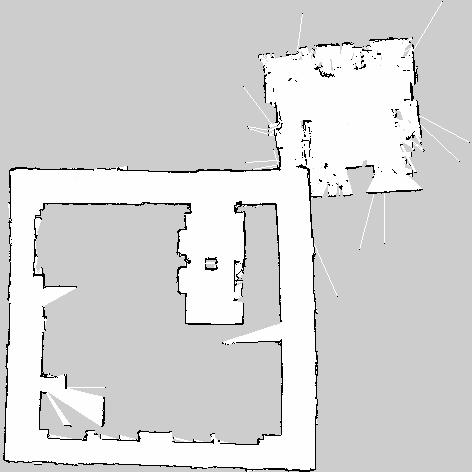
\includegraphics[width=21pc]{map.jpeg}
	\caption{Initial Map}
	\label{fig_env}
	\end{figure}
	\\

\subsection{Localização}

%amcl - localization
%
%RosAria - metapackage with odometry package, communication with robot
%
%hokuyo\_node - laser ranger

\subsection{Navegação}

%navigation stack - navigation
% - move\_base
% - local planner
% - global planner
 
	For doing the Navigation the used commands gived by the user
	\\
	\\
	Odometry:
	\\
	\\
	The pose have tree parameters: x, y , $\theta$
	
	
	
	
	Algorithm:
	
	
	
	
	
	
	
	We use Rosaria to obtain odometry information for doing the localization in the map, the odometry information obtain in topic pose published by Rosaria.
	Another thing we use Rosaria is for reading the sonar, give by the topic sonar.
	\\
	\\

\subsection{Execução do Plano Coordenado}

%smach - finite state automaton
% - actionlib
 
In order to coordinate the robot's actions, an abstract representation of the task to be carried out is needed. The receptionist robot is a sequential system, \textit{i.e.}, it performs one action at a time -- either moving to a target location or interacting with a user to acquire one. For such a system, a State Machine (SM), or Finite State Automaton (FSA) is usually used to specify the control flow through the system.

A SM is implemented using the \textit{smach} package. The task of the robot is divided into three states:
\begin{itemize}
	\item INITIAL
	\item TO\_GOAL
	\item GET\_GOAL
\end{itemize}

\subsection{Interacção com o Utilizador}

%gspeech/pocketsphynx - speech recognition
%
%sound\_play - speech synthesis

\subsection{Visualização}

%Rviz - visualization

The project was developed on the Robot Operating System framework, which is open-source and contains a myriad of different off-the-shelf packages ready for use.

\section{Resultados}
% Experimental Results (show the most relevant results to illustrate the merits and the possible unresoved issues)

\section{Conclusão}
% Conclusions (lessons taken, major conclusions, reasons for what went wrong, if anything)


\appendices
% if have a single appendix:
%\appendix[Proof of the Zonklar Equations]
% or
%\appendix  % for no appendix heading
\section{Title of Appendix A}
Appendix A text goes here.
desired:

\begin{thebibliography}{1}
\bibitem{IEEEhowto:kopka}
	H.~Kopka and P.~W. Daly, \emph{A Guide to \LaTeX}, 3rd~ed.\hskip 1em plus
	0.5em minus 0.4em\relax Harlow, England: Addison-Wesley, 1999.
\end{thebibliography}

\end{document}

%----------------------------

% Floating figure
\begin{figure}[!t]
\centering
\includegraphics[width=2.5in]{myfigure}
\caption{Simulation Results.}
\label{fig_sim}
\end{figure}

% Double column floating figure using two subfigures.
\begin{figure*}[!t]
\centering
\subfloat[Case I]{\includegraphics[width=2.5in]{box}%
\label{fig_first_case}}
\hfil
\subfloat[Case II]{\includegraphics[width=2.5in]{box}%
\label{fig_second_case}}
\caption{Simulation results.}
\label{fig_sim}
\end{figure*}

% Floating table
\begin{table}[!t]
% increase table row spacing, adjust to taste
\renewcommand{\arraystretch}{1.3}
 if using array.sty, it might be a good idea to tweak the value of
 \extrarowheight as needed to properly center the text within the cells
\caption{An Example of a Table}
\label{table_example}
\centering
% Some packages, such as MDW tools, offer better commands for making tables
% than the plain LaTeX2e tabular which is used here.
\begin{tabular}{|c||c|}
\hline
One & Two\\
\hline
Three & Four\\
\hline
\end{tabular}
\end{table}


